\documentclass[journal,12pt,twocolumn]{IEEEtran}

\usepackage{setspace}
\usepackage{gensymb}

\singlespacing


\usepackage[cmex10]{amsmath}

\usepackage{amsthm}

\usepackage{mathrsfs}
\usepackage{txfonts}
\usepackage{stfloats}
\usepackage{bm}
\usepackage{cite}
\usepackage{cases}
\usepackage{subfig}

\usepackage{longtable}
\usepackage{multirow}

\usepackage{enumitem}
\usepackage{mathtools}
\usepackage{steinmetz}
\usepackage{tikz}
\usepackage{circuitikz}
\usepackage{verbatim}
\usepackage{tfrupee}
\usepackage[breaklinks=true]{hyperref}
\usepackage{graphicx}
\usepackage{tkz-euclide}
\usepackage{float}

\usetikzlibrary{calc,math}
\usepackage{listings}
    \usepackage{color}                                            %%
    \usepackage{array}                                            %%
    \usepackage{longtable}                                        %%
    \usepackage{calc}                                             %%
    \usepackage{multirow}                                         %%
    \usepackage{hhline}                                           %%
    \usepackage{ifthen}                                           %%
    \usepackage{lscape}     
\usepackage{multicol}
\usepackage{chngcntr}

\DeclareMathOperator*{\Res}{Res}

\renewcommand\thesection{\arabic{section}}
\renewcommand\thesubsection{\thesection.\arabic{subsection}}
\renewcommand\thesubsubsection{\thesubsection.\arabic{subsubsection}}

\renewcommand\thesectiondis{\arabic{section}}
\renewcommand\thesubsectiondis{\thesectiondis.\arabic{subsection}}
\renewcommand\thesubsubsectiondis{\thesubsectiondis.\arabic{subsubsection}}


\hyphenation{op-tical net-works semi-conduc-tor}
\def\inputGnumericTable{}                                 %%

\lstset{
%language=C,
frame=single, 
breaklines=true,
columns=fullflexible
}
\makeatletter
\setlength{\@fptop}{0pt}
\makeatother
\begin{document}
\newtheorem{theorem}{Theorem}[section]
\newtheorem{problem}{Problem}
\newtheorem{proposition}{Proposition}[section]
\newtheorem{lemma}{Lemma}[section]
\newtheorem{corollary}[theorem]{Corollary}
\newtheorem{example}{Example}[section]
\newtheorem{definition}[problem]{Definition}

\newcommand{\BEQA}{\begin{eqnarray}}
\newcommand{\EEQA}{\end{eqnarray}}
\newcommand{\define}{\stackrel{\triangle}{=}}
\bibliographystyle{IEEEtran}
\providecommand{\mbf}{\mathbf}
\providecommand{\pr}[1]{\ensuremath{\Pr\left(#1\right)}}
\providecommand{\qfunc}[1]{\ensuremath{Q\left(#1\right)}}
\providecommand{\sbrak}[1]{\ensuremath{{}\left[#1\right]}}
\providecommand{\lsbrak}[1]{\ensuremath{{}\left[#1\right.}}
\providecommand{\rsbrak}[1]{\ensuremath{{}\left.#1\right]}}
\providecommand{\brak}[1]{\ensuremath{\left(#1\right)}}
\providecommand{\lbrak}[1]{\ensuremath{\left(#1\right.}}
\providecommand{\rbrak}[1]{\ensuremath{\left.#1\right)}}
\providecommand{\cbrak}[1]{\ensuremath{\left\{#1\right\}}}
\providecommand{\lcbrak}[1]{\ensuremath{\left\{#1\right.}}
\providecommand{\rcbrak}[1]{\ensuremath{\left.#1\right\}}}
\theoremstyle{remark}
\newtheorem{rem}{Remark}
\newcommand{\sgn}{\mathop{\mathrm{sgn}}}
\providecommand{\abs}[1]{\vert#1\vert}
\providecommand{\res}[1]{\Res\displaylimits_{#1}} 
\providecommand{\norm}[1]{\lVert#1\rVert}
%\providecommand{\norm}[1]{\lVert#1\rVert}
\providecommand{\mtx}[1]{\mathbf{#1}}
\providecommand{\mean}[1]{E[ #1 ]}
\providecommand{\fourier}{\overset{\mathcal{F}}{ \rightleftharpoons}}
%\providecommand{\hilbert}{\overset{\mathcal{H}}{ \rightleftharpoons}}
\providecommand{\system}{\overset{\mathcal{H}}{ \longleftrightarrow}}
	%\newcommand{\solution}[2]{\textbf{Solution:}{#1}}
\newcommand{\solution}{\noindent \textbf{Solution: }}
\newcommand{\cosec}{\,\text{cosec}\,}
\providecommand{\dec}[2]{\ensuremath{\overset{#1}{\underset{#2}{\gtrless}}}}
\newcommand{\myvec}[1]{\ensuremath{\begin{pmatrix}#1\end{pmatrix}}}
\newcommand{\mydet}[1]{\ensuremath{\begin{vmatrix}#1\end{vmatrix}}}
\numberwithin{equation}{subsection}
\makeatletter
\@addtoreset{figure}{problem}
\makeatother
\let\StandardTheFigure\thefigure
\let\vec\mathbf
\renewcommand{\thefigure}{\theproblem}
\def\putbox#1#2#3{\makebox[0in][l]{\makebox[#1][l]{}\raisebox{\baselineskip}[0in][0in]{\raisebox{#2}[0in][0in]{#3}}}}
     \def\rightbox#1{\makebox[0in][r]{#1}}
     \def\centbox#1{\makebox[0in]{#1}}
     \def\topbox#1{\raisebox{-\baselineskip}[0in][0in]{#1}}
     \def\midbox#1{\raisebox{-0.5\baselineskip}[0in][0in]{#1}}
\vspace{3cm}
\title{GATE ASSIGNMENT-3}
\author{Vojeswitha Gopireddy \\ AI20BTECH11024}
\maketitle
\newpage
\bigskip
\renewcommand{\thefigure}{\theenumi}
\renewcommand{\thetable}{\theenumi}
Download all python codes from 
\begin{lstlisting}
https://github.com/V-Gopireddy/EE3900/blob/main/GATE_Assignment3/codes/GateAssignment-3.py
\end{lstlisting}

And all latex-tikz from 
%
\begin{lstlisting}
https://github.com/V-gopireddy/EE3900/blob/main/GATE_Assignment3/GateAssignment-3.tex
\end{lstlisting}
\section{QUESTION EC-2001/Q.1.3}
The transfer function of a system is given by 
\begin{align}
  H(s) = \frac{1}{s^2(s-2)}  
\end{align}
The impulse response of the system is
\begin{enumerate}
    \item  $(t2 * e^{-2t})U(t)$
    \item $(t * e^{2t})U(t)$
    \item $(te^{-2t})U(t)$
    \item $(te^{-2t})U(t)$
\end{enumerate}
%
\section{SOLUTION}
%
\begin{lemma}[Table of Laplace Transforms]\label{tbl}
\begin{center}
\begin{tabular}{ |m{4cm}|m{4.5cm}| } 
 \hline
 $\textbf{Time Function}$ $f(t)=\mathcal{L}^{-1}\cbrak{F(s)}$ & $\textbf{Laplace transform}$ of f(t) $F\brak{s}=\mathcal{L}\cbrak{f\brak{t}}$ \\ 
 \hline
 $t^{n}U(t)$, $n \ge 1$ & $\dfrac{n!}{s^{n+1}}$, $s>0$ \\ 
 \hline
 $\dfrac{t^{n-1}}{(n-1)!}U(t)$, $n \ge 2$ & $\dfrac{1}{s^n}$, $s > 0$ \\
 \hline
 $e^{-at}U\brak{t}$ & $\frac{1}{s+a}$, $s+a>0$\\
 \hline
\end{tabular}
\end{center}
\end{lemma}
\begin{theorem}[Convolution theorem]
Suppose $F(s)=\mathcal{L}\cbrak{f(t)}, G(s)=\mathcal{L}\cbrak{g(t)}$ exist, then,
\begin{align}
    \mathcal{L}^{-1}\cbrak{F(s)G(s)}=f(t)*g(t)\label{eq:cuf}
\end{align}
\end{theorem}
Let,
\begin{align}
    F(s) &= \frac{1}{s^2}, G(s) = \frac{1}{s-2}\\
    \implies f(t) &= \mathcal{L}^{-1}\cbrak{\frac{1}{s^2}} = \frac{t}{1!} = tU(t)\\
    \implies g(t) &= \mathcal{L}^{-1}\cbrak{\frac{1}{s-2}} = e^{2t}U(t)
\end{align}
Given transfer function,
\begin{align}
   H(s) &= \frac{1}{s^2(s-2)} \\
   \implies h(t) &=  \mathcal{L}^{-1}\cbrak{H(s)}  \\
   &= \mathcal{L}^{-1}\cbrak{\frac{1}{s^2(s-2)}}\label{eq:1}\\
   &= \mathcal{L}^{-1}\cbrak{F(s)G(s)}\\
   &= f(t)*g(t)
   = (t*e^{2t})U(t)
\end{align}
Correct Option is (2)
\begin{figure}[!h]
         \centering
         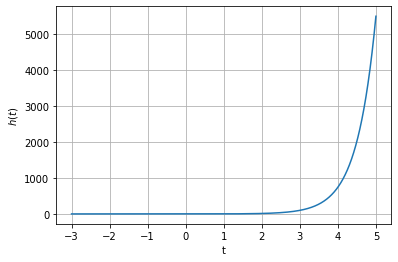
\includegraphics[width=\columnwidth]{h(t)-plot.png}
         \caption{Plot of $h(t) = (t*e^{2t})U(t)$}
         \label{plot}
\end{figure}
\end{document}